\documentclass[a4paper,hidelinks]{article}
\usepackage{bnaic}
\usepackage[T1]{fontenc}
\usepackage[utf8]{inputenc}
\usepackage{natbib}

\usepackage{filecontents}
\usepackage{hyperref}
\usepackage{graphicx}


\title{\textbf{\huge Traffic Memory: A Multi Agent System Approach to Traffic Flow Optimization}%
}
\author{
	Wouter Reckman (s2231166) \and
    Matthia Sabatelli (s2847485) \and
    Gereon Vienken (s2738805) 
}
\date{}

\pagestyle{empty}

\begin{document}
\ttl
\thispagestyle{empty}

%\bibliography{dmas-gereon_matthia_wouter-traffic_memory-report}


\begin{abstract}
\noindent
In this paper we present a Multi-Agent System simulation of traffic in which 147 agents travel for 10 days in a 7x7 grid, moving from a randomized starting position to a randomly assigned destination. The grid symbolizes a Manhattan-like city consisting of junctions. The number of agents able to move through these junctions during each (discrete) time step is limited, thus creating bottlenecks which in turn may cause traffic jams. This regards the first part of the experiment, in the second part we provide the agents with a memory system enabling them to remember the most congested junctions. Using a weighted A* path finding algorithm they can avoid these and potentially the amount of traffic jams occurring could be reduced. Our results however, showed the opposite effect, which we attribute to a form of cut-through driving arising.
\end{abstract}


\section{Introduction}
During the past decades, travel by car has always been one of the most comfortable and appreciated ways to move through countries and the amount of traffic is ever increasing. Several reasons of this constant growth can be indicated, ranging from the constant increase of affordability of cars, enabling almost every family to own one or several cars, to the creation of the European Community which has led to the elimination of boundaries between countries and has facilitated the trade and exchange of resources between different nations.

As a result, millions of people suffer everyday from congestion and traffic jams in urban road networks while travelling to their daily destinations. Possibly, this happens due to existing road networks and the traffic light systems being outdated and not up to the task of regulating the vastly increased quantity of car traffic of the 21st century. Another possible cause is the tendency of drivers occupying these road networks to exhibit selfish behaviour instead of cooperating to make traffic flow more liveable.

It is desirable to minimize the amount of traffic congestions, because it has several negative impacts. Firstly, it leads to frustration and selfish or even aggressive behaviour of traffic participants in an attempt to move through the traffic faster. \\
Secondly, exhaust gases have a severe negative ecological impact on the environment. Air pollution has in fact reached such high levels that in some countries it has been identified as one of the main reasons of the exacerbation of asthma, allergy and many other respiratory diseases. Part of the air pollution is caused by the auto mobile exhausts that, combined with certain industrial pollutants, produce photochemical reactions which in turn damage human health \cite{ghose2005assessment}. \\
Even though most people do not think about all these issues, traffic has a very important role in society and this has led to the work that is presented in the next sections.


\subsection{Problem}
As already mentioned the main problem we try to address regards the inefficiencies in traffic. A lot of research has been done in this field by various scientists and as it will be explained more in detail in the state of the art section the flow of traffic has been modelled under various conditions in order to measure its relative impact. This paper tries to add to this reservoir by trying to understand which possible impact the driver memory of different agents that deal with repeating traffic situations may have. In fact, we all know the situation of drivers that face traffic jams on their daily commute, but what we would like to investigate is how these drivers face jams at the same junction day after day, will they still decide to drive the same route and make the situation on the streets even more worse then it actually is or would they better it by deciding to try their luck of the beaten path the next time? This article tries to get closer to an answer for these questions. 

\subsection{State of the art}
Several research that deals with the optimization of traffic flow may be found in literature and mainly it is possible to divide the approaches that guide this type of research into two sub-fields which both naturally suit the artificial intelligence agent paradigm: on the one side there is research that focuses on modelling the single agents that are on the street; the main idea of this approach is that by modifying their behaviours the whole situation of the traffic will change as a consequence. This approach may be defined as reductionistic since it deals with the single agents on the streets in order to get an overall improvement of the whole traffic flow. On the other side there is research that tries to model the overall behaviour on the streets without directly influencing the single agents, this is done by putting focus on external agents that govern traffic as the most common traffic lights. This last category is for sure the most intuitive and easy to understand one since in everyday life we deal with traffic lights continuously. In fact it does not need to be an expert to understand how a traffic light system works. There is in fact a traffic signal timing plan where various traffic phases are coordinated by the traffic light system itself, this is done in order to prevent crashes between traffic phases and ensure the smoothness of the overall traffic flow within the traffic network. As explained in [1] there are various ways in which these kind of systems may work but the most general idea is that there is a fixed-time traffic signal plan management where all the duration of the traffic signals are pre-set in the database and being executed repeatedly. The configurations of he traffic signals durations are done based on some historical traffic statistic gathered for a long period. The setting of the fixed time traffic signal plan is then not changed until the next review on the statistic traffic information is provided. This is a very common approach but as highlighted in the paper a little bit too static, in order to better the way in which the traffic light system works the authors have provided the system with a reinforcement learning algorithm that makes it able to adapt itself to the traffic flow it deals with. This is for sure a possible way to model traffic flow but this paper has been inspired by the first possible approach that was explained before, in fact the main article that guided our work was proposed by Gabel et al. in 2008 \cite{gabel2012cooperative}. In this paper the authors compared two microscopic traffic simulations that regarded two types of possible drivers: one selfish driver model and one selfless driver model. They showed that the selfish driver simply tried to maximize his own speed without caring about the rest of the drivers and the general situation of the roads, doing so the probability that traffic jams occurred was very high since there was not any cooperation by the various agents on the streets. On the other side the selfless drivers used a Markov decision model in order to maximize the speed over all cars, doing so it is true that every agent tried to minimize his personal costs but at the same time he does this bearing in mind that there are other agents as well on the streets and is able to find a compromise in order to do not get stacked in the traffic. We were very inspired by this approach that tries to verify the impact of another human trade in traffic simulations. As will be explained more in detail in the next sessions of this paper we decided to provide our agents with a memory system that allowed them to remember situations in which they had to deal with traffic jams, bearing these in mind they are able to come up with different driving strategies that may be a little bit less fast but that optimize the general traffic flow of the streets.
This kind of compromise may be seen in different research papers as mentioned by France et al. \cite{france2003multiagent} coordination between the different agents on the streets is in fact of key importance since it is crucial to maintain a balance between optimized events both at a global level then at a local one. Unfortunately this kind of approach is also very difficult to implement since optimizing local events does not necessarily guarantee a global balance.         

\subsection{New idea}
The new idea of our project proposal is to see if memory can actually have an impact on the flow of traffic over longer periods of time. Thinking about this project we came up with the idea that this may also deal with theory of mind but this link is not directly mentioned in this work, however it may provide an interesting approach for further research. This paper has been guided by the hope that our implementation can show that with providing the agents with some memory in order to avoid previously encountered situations, the traffic flow over the map will go smoother and that the average travelling speed per car will increase. Moreover it is important to highlight that in contrast to our main reference paper \cite{gabel2012cooperative} we only use selfish agents, but by making them more intelligent to pursue their own goals we hope that as an indirect result they will help other agents in the overall process as well.

\section{Method}
\subsection{Simulation model}
To make our traffic simulation we have defined and implemented the following parameters. A 7x7 grid in which a total of 147 independent agents travel from a random chosen starting point to a random chosen destination. They do this for 10 days without interruption and try to get to their destination as quickly as possible using the A* path finding algorithm. We have divided each day in 30 timestamps in which the agents have the chance to end up to their destination, once they arrive they restart the next day with the same parameters over and over. In this grid there are 49 junctions they can travel through which have a certain agent capacity that we have setted to 3, once this limit is reached the traffic gets blocked and traffic jams occur. This scenario is explained in the figure hereafter where the more red the junction gets the more blocked the traffic turns out to be:

\begin{figure}[ht!]
\centering
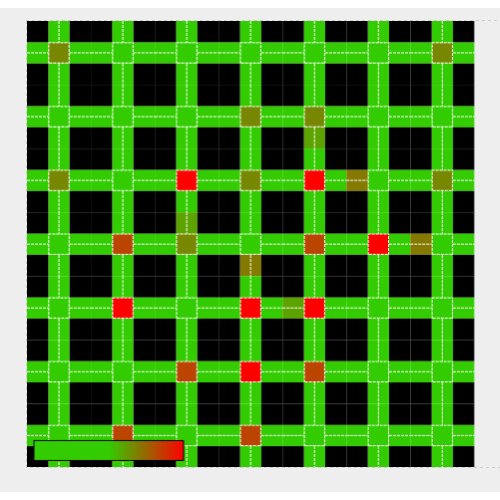
\includegraphics[width = 0.7\linewidth]{grid}
\caption{Traffic Scenario \label{overflow}}
\end{figure} 


These traffic jams can occur if cars first try to enter a junction from more directions and then will try to leave it simultaneously, this turns the junction into a kind of bottleneck. This aspect of the traffic is on what our whole simulation goes about. At the end of the first 10 days simulation our agents remember the junctions in which the more traffic occurred and in the second part of it they use this information to re-plan their routes in our version of the A* algorithm. This means that the path finding algorithm gives different weights to the various steps it has computed to make an agent get to his destination, in fact if one of these steps corresponds to a high congested junction the algorithm plans a new route in which he tries to avoid it. We have decided to go with a global memory model since on one side it is easier to implement and on the other side it is more human likely since it reflects the fact that these information is actually available for every driver that deals with a very common navigation system. 

\subsection{Experiment design}

As already explained we have divided our whole simulation into 2 parts, the first one is preparatory for the second one since it is where the agents acquire the memory knowledge they will need in the second one in order to improve the traffic flow. During the 10 days of the 2 simulations we have measured and tracked the following parameters for every agent. First of all the starting point and the destination point that have been randomly assigned in order to get an idea where the agents needed to go. We also have measured the relocation process in order to see if and how they are moving, but the most important data comes from the Stuck TS parameter that measures how much each agent that is blocked in traffic is waiting before being able to reach its destination. We also have kept track of the overall distance that each agent has covered during its travelling period, the highest this parameter is, the more likely it is that the agent has bumped into a traffic jam. These parameters are all shown in the following figure:

\begin{figure}[ht!]
\centering
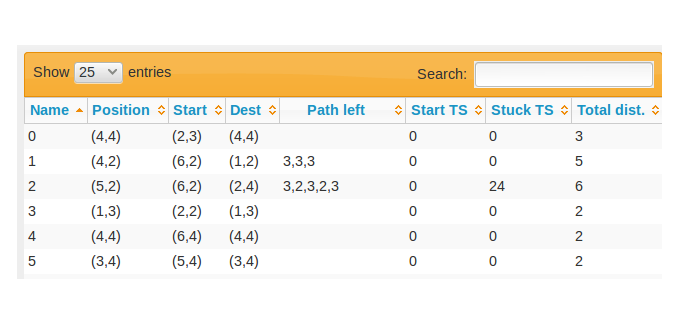
\includegraphics[width = 1.0\linewidth]{data}
\caption{Measurements Table \label{overflow}}
\end{figure} 


\section{Results}
\subsection{Experiment findings}
The main data we were interested in is the percentage of jams occurring during the two parts of the simulation, that namely refer to the agents travelling with the normal A* algorithm and with the weighted version of it that simulates the memory. During our computational simulation we have saved the amount of jams that have occurred for every time step for a period of 10 days and this has been done for 100 times. So we have calculated the amount of jams, for each time step (30) for 10 days. This has been repeated for 100 times. This has been done in order to be able to compute an average representing the occurrence of the traffic jams over a decent amount of data. In the next section the graphs that represent this simulation are discussed in order to show how the amount of jams has decreased over time when the agents were provided with memory.  

\begin{figure}[ht!]
\centering
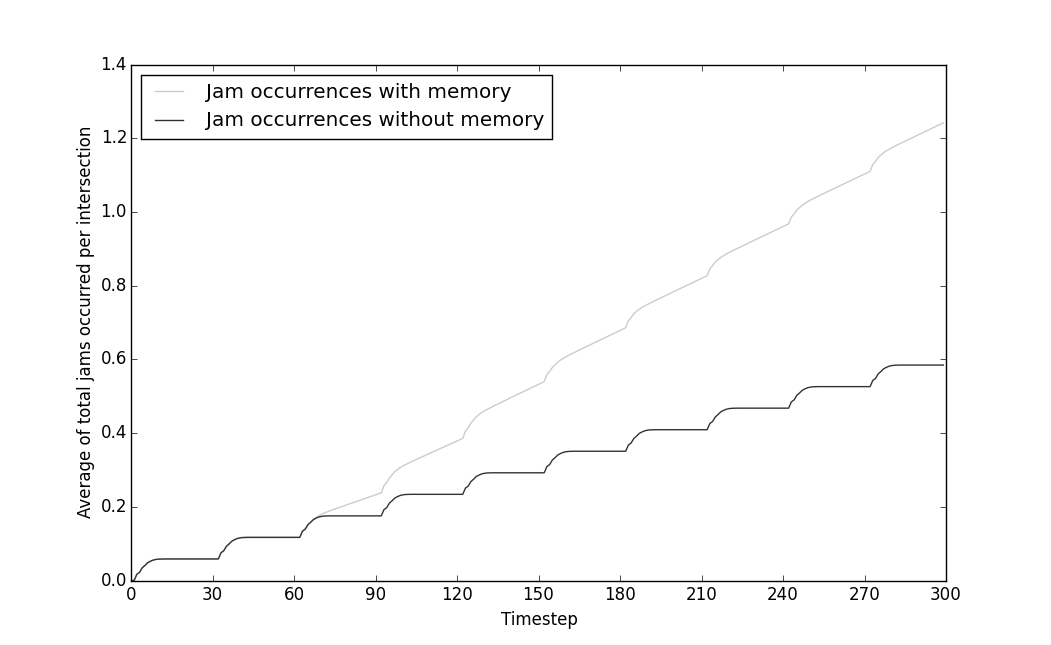
\includegraphics[width = 0.7\linewidth]{100sims-mem-vs-nomem}
\caption{Progression of traffic jams over time\label{overflow}}
\end{figure} 

\subsection{Interpretation of findings}
What's the story? Why is happening what is happening? verwacht: sluiproutegedrag, en ToM nodig om dat te vermijden

\section{Conclusion}
\subsection{Discussion}
\subsection{Relevance}
The intention of this paper was to show, that the use of memory in a repeated traffic situation can improve traffic flow and prevent traffic jams. This information could be used to improve traffic guidance systems like GPS. If memory improves the traffic flow even though its just agent independent knowledge, that would mean, that a selfish change in behaviour can still improve the traffic situation as a whole without the need of direct inter-agent communication. If this is not possible it would be necessary for the agents to communicate with one another in order to distribute the traffic intentionally which would require a large amount of work and inter cooperation-cooperation. The benefit of an easy solution could guarantee, that improved guiding systems could be produced that by their usage would optimize traffic for everyone. The benefits of optimised traffic are wildly known \cite{france2003multiagent}. Not just that it's bad for your personal health when you come to work with high bloodstream and the intend to murder people, but it's also unproductive for thousands of people to spend hours a day doing nothing. On a global scale, optimising traffic also has the beneficial trade to reduce the carbon emission of the cars, that no longer stand on the streets with running motors. All in all, optimising traffic is a worthwhile attempt to promote peoples health productivity and quality of life. 

\section{Acknowledgements}

\bibliographystyle{plain}
\bibliography{dmas-gereon_matthia_wouter-traffic_memory-report.bib}


\end{document}
